\documentclass[9pt]{beamer}
\usetheme{metropolis}
%\usetheme{Warsaw}
\metroset{titleformat=smallcaps,block=fill}
\usecolortheme{seahorse}
%\usepackage[utf8]{inputenc}
\usepackage[spanish]{babel}
\usepackage{amsmath}
\usepackage{amsfonts}
\usepackage{amssymb}
\usepackage{graphicx}
\usepackage{tikz} 
\usetikzlibrary{matrix}
\usetikzlibrary{calendar,decorations.markings} 
\usetikzlibrary{shapes,positioning}

\usepackage{tkz-tab,tkz-euclide,tkz-fct}

\usetkzobj{all} 
\usepackage{polynom}

\newcommand{\R}{\mathbb{R}}

\author{Departamento de Matemáticas}
\title{Determinantes}
%\subtitle{Definición y cálculo}
%\setbeamercovered{transparent} 
%\setbeamertemplate{navigation symbols}{} 
%\logo{
\includegraphics[scale=0.05]{../../images/logoa.jpg}} 
%\institute{UHEI - IVED} 
\date{
\includegraphics[scale=0.15]{imagenes/logoa.jpg}} 
%\subject{} 
\begin{document}

\begin{frame}
\titlepage
\end{frame}

\begin{frame}
\tableofcontents
\end{frame}

\section{Determinantes}

\begin{frame}{Calculo de determinantes}

\begin{alertblock}{Determinante de orden 2}
Dada una matriz de orden 2,$A=\begin{pmatrix}
a_{11}& a_{12}  \\
a_{21} & a_{22} 
\end{pmatrix}$, se llama determinante de $A$ al número real : 

\[ det(A)= |A|= \begin{vmatrix}
a_{11}& a_{12}  \\
a_{21} & a_{22} 
\end{vmatrix}=a_{11} \cdot a_{22}-a_{12}\cdot a_{21} \]
\end{alertblock}
   \begin{exampleblock}{Ejemplo}
   $\begin{vmatrix}
1& 3  \\
2 &5 
\end{vmatrix}=1\cdot 5-3\cdot 2=-1 $
   \end{exampleblock}
\end{frame}

\begin{frame}{Determinante de orden 3}
\begin{alertblock}{Determinante de orden 3}
Dada una matriz de orden 3,$A=\begin{pmatrix}
a_{11}& a_{12} & a_{13} \\
a_{21} & a_{22} & a_{23} \\
a_{31}& a_{32} & a_{33}
\end{pmatrix}$, se llama determinante de $A$ al número real : 

\[ det(A)= |A|= \begin{vmatrix}
a_{11}& a_{12}  &a_{13} \\
a_{21} & a_{22}&a_{23}\\
a_{31} & a_{32}&a_{33}
\end{vmatrix} = \]
\[ =a_{11} \cdot a_{12} \cdot a_{13}+a_{12} \cdot a_{23} \cdot a_{31}+a_{13} \cdot a_{32} \cdot a_{21}-a_{13} \cdot a_{22} \cdot a_{31}-a_{23} \cdot a_{32} \cdot a_{21}-a_{33} \cdot a_{21} \cdot a_{12} \]
\end{alertblock}

Para recordar estos productos podemos utilizar la regla de Sarrus:
\begin{figure}[h]
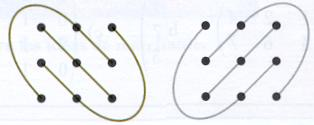
\includegraphics[scale=0.7]{imagenes/sarrus.jpg}
\end{figure}

\end{frame}


\begin{frame}{Determinantes de orden 3}
\begin{exampleblock}{Ejemplo}
Calcular el siguiente determinante:
$\begin{vmatrix}1&2&3\\
0&-1&2\\
2&1&3
\end{vmatrix}$
\end{exampleblock}
\pause
Aplicamos la regla de Sarrus:

\begin{figure}[h]
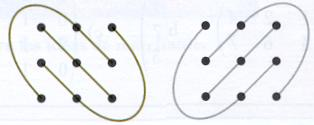
\includegraphics[scale=0.7]{imagenes/sarrus.jpg}
\end{figure}


$\begin{vmatrix}1&2&3\\
0&-1&2\\
2&1&3
\end{vmatrix}$\pause $=1\cdot (-1) \cdot 3$\pause $ +2\cdot 2 \cdot 2$\pause $+ 3\cdot 1 \cdot 0 $\pause  $-3\cdot (-1)\cdot 2 $\pause $- 2\cdot 0\cdot 3 $\pause $- 1\cdot 1 \cdot 2$\pause $=9$

\end{frame}

\section{Propiedades de los determinantes}
\begin{frame}{Propiedades de los determinantes}

\onslide*<1>{Estas propiedades son válidas para determinantes de cualquier orden pero en los ejemplos usaremos determinantes de orden$3$}

\onslide*<2>{El determinante de una matriz y el de su traspuesta son iguales. Las propiedades valen indistintamente para filas o columnas.
$$\vert A \vert =\vert A^t \vert $$ }


\onslide*<3>{Si todos los elementos de una linea de un determinante son ceros, el determinante también es cero.
$$\begin{vmatrix}
1&0&2\\
2&0&4\\
-1&0&3
\end{vmatrix}=0$$}

\onslide*<4>{Si en un determinante se intercambian dos lineas, el determinante cambia de signo.
$$\begin{vmatrix}
3&-2&5\\
1&7&3\\
4&1&0
\end{vmatrix}=-168\longrightarrow \begin{vmatrix}
1&7&3\\
3&-2&5\\
4&1&0
\end{vmatrix}=-(-168)=168$$}

\onslide*<5>{ Si en un determinante dos lineas son iguales, el determinante es cero.
$$\begin{vmatrix}
1&2&1\\
3&-5&3\\
-2&6&-2
\end{vmatrix}=0$$}

\onslide*<6>{ Si los elementos de una linea se multiplican por un número, el determinante también se multiplica por ese número.
$$\begin{vmatrix}
1&5\cdot 7&0\\
-2&3\cdot 7 &4\\
3&7\cdot 7& -1
\end{vmatrix}=7\begin{vmatrix}
1&5&0\\
-2&3 &4\\
3&7& -1
\end{vmatrix}$$}

\onslide*<7>{Si en un determinante dos lineas son proporcionales, el determinante es cero.
$$\begin{vmatrix}
1&5&0\\
-2&3 &4\\
2&10& 0
\end{vmatrix} \stackrel{F_{3}=2 \cdot F_{1}}{=}0$$}

\onslide*<8>{Si los elementos de una línea se pueden descomponer en dos sumandos,  su determinante es igual a la suma de dos determinantes que tienen iguales todas las líneas excepto la línea cuyos sumandos pasan, respectivamente, a cada uno de los determinantes. 
$$\begin{vmatrix}
a_{11}& a_{12}+ a'_{12} &a_{13} \\
a_{21} & a_{22}+a'_{22}&a_{23}\\
a_{31} & a_{32}+a'_{32}&a_{33}
\end{vmatrix}=\begin{vmatrix}
a_{11}& a_{12} &a_{13} \\
a_{21} & a_{22}&a_{23}\\
a_{31} & a_{32}&a_{33}
\end{vmatrix}+\begin{vmatrix}
a_{11}&  a'_{12} &a_{13} \\
a_{21} & a'_{22}&a_{23}\\
a_{31} & a'_{32}&a_{33}
\end{vmatrix}$$}

\onslide*<9>{ Si a una linea de un determinante se le suma una combinación lineal de las demás lineas, el valor del determinante no varía.
$$\begin{vmatrix}
1&5&1\\
-2&3 &4\\
2&10& 3
\end{vmatrix} \stackrel{C_{2}+C_{1}-C_{3}}{=}\begin{vmatrix}
1&5&1\\
-2&-3 &4\\
2&9& 3
\end{vmatrix} $$}

\onslide*<10>{Si en una determinante una linea es combinación lineal de las demás el valor del determinante es cero.
$$\begin{vmatrix}
1&3&4\\
2&3 &5\\
2&-3&-1
\end{vmatrix} \stackrel{C_{3}=C_{1}+C_{2}}{=}0$$}

\onslide*<11>{El determinante del producto de dos matrices cuadradas es igual al producto de los determinantes de ambas matrices 
$$\vert A \cdot B\vert=\vert A \vert\cdot \vert B\vert$$}
 
\end{frame}

\begin{frame}{Ejemplo}
\onslide*<1>{
\begin{exampleblock}{Ejemplo}
 Sabiendo que 
 $ \begin{vmatrix}
 a & b & c \\
 1 & 1 & 1 \\
 3 & 0 & 1
 \end{vmatrix}= 2 $
 calcula, usando las propiedades de los determinantes,
$ \begin{vmatrix}
 3-a & -b & 1-c \\
 1+a & 1+b & 1+c \\
 3a & 3b & 3c 
 \end{vmatrix}
 \qquad \text{y} \qquad 
 \begin{vmatrix}
  2a & 2b & 2c \\
 30 & 0 & 10 \\
  4 & 4 & 4
 \end{vmatrix} $
\end{exampleblock}
}

\onslide*<2-8>{
$
\begin{vmatrix}
 3-a & -b & 1-c \\
 1+a & 1+b & 1+c \\
 3a & 3b & 3c 
 \end{vmatrix}$ }
 \onslide*<3-8>{$ = 
 \begin{vmatrix}
 3 & 0 & 1 \\
 1+a & 1+b & 1+c \\
 3a & 3b & 3c 
 \end{vmatrix}+\begin{vmatrix}
 -a & -b & -c \\
 1+a & 1+b & 1+c \\
 3a & 3b & 3c 
 \end{vmatrix} =  $
\onslide*<4-8>{
 $ \begin{vmatrix}
 3 & 0 & 1 \\
 1+a & 1+b & 1+c \\
 3a & 3b & 3c 
 \end{vmatrix} +  0 (F_3=-3F_1)$}
\onslide*<5-8>{ $ = 
 \begin{vmatrix}
 3 & 0 & 1 \\
 1 & 1 & 1 \\
 3a & 3b & 3c 
 \end{vmatrix}+ \begin{vmatrix}
 3 & 0 & 1 \\
 a & b & c \\
 3a & 3b & 3c 
 \end{vmatrix} $}
 \onslide*<6-8>{$ \begin{vmatrix}
 3 & 0 & 1 \\
 1 & 1 & 1 \\
 3a & 3b & 3c 
 \end{vmatrix}+  0 (F_3=3F_2) $}
 \onslide*<7-8>{$ = 3\begin{vmatrix}
 3 & 0 & 1 \\
 1 & 1 & 1 \\
 a & b & c 
 \end{vmatrix}$}
  \onslide*<8>{ $= -3 \begin{vmatrix}
 a & b & c\\
 1 & 1 & 1 \\
   3 & 0 & 1
 \end{vmatrix} = -6 
$}
}

\onslide*<9>{
\begin{eqnarray*}
\begin{vmatrix}
  2a & 2b & 2c \\
  30 & 0 & 10 \\
 4 & 4 & 4
 \end{vmatrix} &=&   2\cdot 10 \cdot 4 \begin{vmatrix}
 a & b & c \\
 3 & 0 & 1 \\
 1 & 1 & 1
 \end{vmatrix} = 800  
\end{eqnarray*}
}

\end{frame}
\section{Matriz adjunta}
\subsection{Menor complementario y adjunto}
\begin{frame}{Menor complementario}

\begin{alertblock}{Menor complementario}
Dada una matriz cuadrada de orden $n$, $A=(a_{ij})$, se llama menor complementario del elemento $a_{ij}$ al determinante de orden $n-1$ que se obtiene al eliminar la fila $i$ y la columna $j$ de la matriz $A$. Se suele representar por $M_{ij}$.
\end{alertblock}

\end{frame}

\begin{frame}
\begin{exampleblock}{Ejemplo}
Dada la matriz $A=\begin{pmatrix} 
1 & -2 & 3 \\
-1 & 0 & 2 \\
-2 & 3 & -1 \\
\end{pmatrix}$, hallar los menores complementarios $M_{12}$, $M_{22}$ y $M_{31}$
\end{exampleblock}
\pause
Para hallar los menores complementarios formamos los determinantes de orden $2$, ya que la matriz es de orden $3$, que resultan de eliminar la fila y la columna correspondiente.
\pause
\[ 
M_{12}=\begin{vmatrix}  -1 & 2 \\ -2 & -1 \\ \end{vmatrix}=5 \]
\[ M_{22}=\begin{vmatrix}  1 & 3 \\ -2 & -1 \\ \end{vmatrix}=4 \]
\[M_{31}=\begin{vmatrix}  -2 & 3 \\ 0 & 2 \\ \end{vmatrix}=-4
\]

\end{frame}

\begin{frame}{Adjunto}
\begin{alertblock}{Adjunto}
Dada una matriz cuadrada de orden $n$, $A=(a_{ij})$, se llama adjunto del elemento $a_{ij}$ al menor complementario de dicho elemento precedido del signo $+$ o $-$, según si la suma de $i+j$ es par o impar. Se suele representar por $A_{ij}$.
\[
A_{ij}=(-1)^{i+j} \cdot M_{ij}
\]
\end{alertblock}
\end{frame}

\begin{frame}{Adjunto}
\begin{exampleblock}{Ejemplo}
Dada la matriz $A=\begin{pmatrix} 
 1& -2& 3 \\
 -1& 0& 2 \\
 -2& 3& -1 \\
\end{pmatrix}$, hallar los adjuntos $A_{12}$, $A_{22}$ y $A_{31}$
\end{exampleblock}
\pause
Para hallar los adjuntos anteponemos el signo $+$ o $-$ a los menores correspondientes (calculados en el ejemplo anterior).
\pause
\[
A_{12}=(-1)^{1+2} \cdot M_{12}=-5 \qquad A_{22}=(-1)^{2+2} \cdot M_{22}=4 \qquad A_{13}=(-1)^{1+3} \cdot M_{31}=-4
\]
\end{frame}
\subsection{Matriz adjunta}

\begin{frame}{Matriz adjunta}
\begin{alertblock}{Matriz adjunta}
Se llama matriz adjunta de una matriz cuadrada $A(a_{ij})$ a la matriz que resulta de cambiar cada elemento $a_{ij}$ de la matriz por el adjunto de ese elemento $A_{ij}$. Se representa por $Adj(A)$.
\end{alertblock}

\end{frame}

\begin{frame}{Matriz adjunta}
\begin{exampleblock}{Ejemplo}
Dada la matriz $A=\begin{pmatrix} 
 1& -2& 3 \\
 -1& 0& 2 \\
 -2& 3& -1 \\
\end{pmatrix}$, hallar su matriz adjunta
\end{exampleblock}
\pause
Calculamos el adjunto de cada elemento.
\pause
\[
\begin{aligned}
A_{11}= + \begin{vmatrix} 0& 2 \\ 3& -1 \\ \end{vmatrix} =   -6 \quad & 
A_{12}= - \begin{vmatrix} -1& 2 \\ -2& -1 \\ \end{vmatrix} =   -5 & 
A_{13}=  + \begin{vmatrix} -1& 0 \\ -2& 3 \\ \end{vmatrix} =   -3 \\
A_{21}= - \begin{vmatrix} -2& 3 \\ 3& -1 \\ \end{vmatrix} =   7 \quad &  
A_{22}= + \begin{vmatrix} 1& 3 \\ -2& -1 \\ \end{vmatrix} =   5 &  
A_{23}= - \begin{vmatrix} 1& -2 \\ -2& 3 \\ \end{vmatrix} =   1 \\
A_{31}= + \begin{vmatrix} -2& 3 \\ 0& 2 \\ \end{vmatrix} =   -4 \quad &
A_{32}=- \begin{vmatrix} 1& 3 \\ -1& 2 \\ \end{vmatrix} =   -5 &
A_{33} + \begin{vmatrix} 1& -2 \\ -1& 0 \\ \end{vmatrix} =   -2 \\
\end{aligned}
\]
\pause
Para obtener la matriz adjunta cambiamos cada elemento por su adjunto.
\pause
\[
Adj(A)=
\begin{pmatrix}
  -6 &  -5  &  -3 \\
  7 &  5&  1 \\
  -4&  -5&  -2 \\
\end{pmatrix}
\]
\end{frame}

\section{Desarrollo de un determinante por adjuntos}
\begin{frame}{Desarrollo determinantes por adjuntos}
\begin{alertblock}{Desarrollo determinantes por adjuntos}
El determinante de una matriz cuadrada de orden $n$ es igual a la suma de los productos de cada elemento de esa fila por sus adjuntos respectivos.

$det(A)= a_{i1}\cdot A_{i1}+a_{i2}\cdot A_{i2}+\cdots +a_{in}\cdot A_{in}$

$det(A)= a_{1j}\cdot A_{1j}+a_{2j}\cdot A_{2j}+\cdots +a_{nj}\cdot A_{nj}$
\end{alertblock}
\end{frame}

\begin{frame}{Desarrollo determinantes por adjuntos}
\begin{exampleblock}{Ejemplo}
Hallar el determinante de la matriz $A=\begin{pmatrix} 
 1& -2& 3 \\
 5& 0& 6 \\
 -1& 2& -4 \\
\end{pmatrix} $
\begin{enumerate}
\item Por la regla de Sarrus.
\item Desarrollando por la primera fila.
\item Desarrollando por la segunda columna.
\end{enumerate}
\end{exampleblock}
\pause
\begin{enumerate}[<+-|alert@+>]
\item $det(A)= 0+12+30-0-12-40=-10$
\item $det(A)=1\cdot \begin{vmatrix}& 0& 6 \\& 2& -4 \\ \end{vmatrix} -(-2)\cdot \begin{vmatrix}& 5& 6 \\& -1& -4 \\ \end{vmatrix} +3\cdot \begin{vmatrix}& 5& 0 \\& -1& 2 \\ \end{vmatrix}= -12-28+30=-10$
\item $det(A)=-(-2)\cdot \begin{vmatrix}& 5& 6 \\& -1& -4 \\ \end{vmatrix} +0\cdot \begin{vmatrix}& 1& 3 \\& -1& -4 \\ \end{vmatrix} -2\cdot \begin{vmatrix}& 1& 3 \\& 5& 6 \\ \end{vmatrix}= -28+0+18=-10$
\pause
En la practica, antes de calcular el determinante, hacemos cero el mayor número posible de elementos de una fila,utilizando las propiedades de los determinantes, y desarrollamos por los elementos de esa fila.

\end{enumerate}
\end{frame}

\begin{frame}{Desarrollo determinantes por adjuntos}

\begin{exampleblock}{Ejemplo}
Hallar el determinante de la matriz $A=\begin{pmatrix} 
 2& 5& -3& -2 \\
 -2& -3& 2& -5 \\
 1& 3& -2& 2 \\
 -1& -6& 4& 3 \\
\end{pmatrix} $
haciendo ceros.
\end{exampleblock}

$det(A)=\begin{vmatrix} 
2 & 5 & -3 & -2 \\
-2 & -3 & 2 & -5 \\
1 & 3 & -2 & 2 \\
-1 & -6 & 4 & 3 \\ \end{vmatrix} \pause
{\color{red}\begin{array}{l} F_1  = F_1+2F_4 \\ F_2=F_2-2F_4 \\ F_3=F_3+F_4 \end{array}} = \pause \begin{vmatrix} 
0 & -7 & 5 & 4 \\
0 & 9 & -6 & -11 \\
0 & -3 & 2 & 5 \\
-1 & -6 & 4 & 3 \\ 
\end{vmatrix} \pause = 
(-1)(-1)^{4+1}\begin{vmatrix} 
-7 & 5 & 4 \\
9 & -6 & -11 \\
-3 & 2 & 5 \\ 
\end{vmatrix} \pause {\color{red}F_2=F_2+3F_3} \pause = 
\begin{vmatrix} 
-7 & 5 & 4 \\
0 & 0 & 4 \\
-3 & 2 & 5 \\ 
\end{vmatrix}\pause = 4\cdot (-1)^{2+3} \begin{vmatrix} 
-7 & 5  \\
-3 & 2  \\ 
\end{vmatrix}\pause = -4(-14+15)=-4
$
\end{frame}
\end{document}
